\documentclass[10pt, aspectratio=169]{beamer}
\usetheme[]{AAUsimple}

\usepackage[utf8]{inputenc}
\usepackage[english]{babel}
\usepackage[T1]{fontenc}
\usepackage{helvet}
\usepackage[style=authoryear, backend=biber]{biblatex}
\usepackage{tikz}
\usetikzlibrary{shapes.geometric, arrows}

% --- AAU Secondary Color Definitions ---
\definecolor{aauDarkOrange}{RGB}{187, 91, 23}
\definecolor{aauDarkGold}{RGB}{151, 112, 31}
\definecolor{aauDarkBlue}{RGB}{0, 127, 163}
\definecolor{aauDarkGreen}{RGB}{14, 133, 99}
\definecolor{aauLightBlue}{RGB}{49, 169, 193}

% colored hyperlinks
\newcommand{\chref}[2]{%
  \href{#1}{{\usebeamercolor[bg]{AAUsimple}#2}}% 
}

\title{Modularity and Geography in Innovation Systems}
\subtitle{A PhD Project Framework}
\date{\today}

\author{
  Roman Jurowetzki
}

\institute[
  Aalborg University Business School\
  Denmark
]
{
  Aalborg University Business School\
  Denmark
}

\pgfdeclareimage[height=1.5cm]{titlepagelogo}{AAUgraphics/aau_logo_new}
\titlegraphic{
  \pgfuseimage{titlepagelogo}
}
\addbibresource{references.bib}

\begin{document}

{\aauwavesbg%
\begin{frame}[plain,noframenumbering]
  \titlepage
\end{frame}}

\begin{frame}{The Core Puzzle}
    \begin{block}{The fundamental research question}
        How does a technology's internal architecture shape the optimal geography of its innovation system?
    \end{block}
    
    \vfill
    
    \begin{columns}[T]
        \begin{column}{.48\textwidth}
            \textbf{When should policy be \textcolor{aauDarkBlue}{local}?}
            \begin{itemize}
                \item Fostering clusters & tacit knowledge
                \item For tightly integrated, complex systems
                \item Building regional advantages
            \end{itemize}
        \end{column}
        \begin{column}{.48\textwidth}
            \textbf{When should policy be \textcolor{aauDarkOrange}{global}?}
            \begin{itemize}
                \item Aligning standards & value chains
                \item For modular systems with clear interfaces
                \item Leveraging international knowledge
            \end{itemize}
        \end{column}
\end{columns}
    
    \vfill
    \centering
    \textbf{This project argues that the answer lies in the technology itself.}
\end{frame}

\begin{frame}{Theoretical Toolkit}
    \textbf{We build on three streams of literature to connect technology, innovation, and policy:}
    
    \vfill
    
    \begin{columns}[T]
        \begin{column}{.32\textwidth}
            \begin{block}{\textcolor{aauDarkBlue}{1. Modularity Theory}}
                Provides the lens to understand a technology's architecture. Modular designs allow parts to be developed independently and recombined \parencite{baldwin2000design}.
            \end{block}
        \end{column}
        
        \begin{column}{.32\textwidth}
            \begin{block}{\textcolor{aauDarkGreen}{2. Innovation Systems (TIS/GIS)}}
                Provides the tools to measure innovation activity and geography, tracking functions like knowledge creation and market formation \parencite{hekkert2007functions, binz2017global}.
            \end{block}
        \end{column}
        
        \begin{column}{.32\textwidth}
            \begin{block}{\textcolor{aauDarkOrange}{3. Policy Mix Theory}}
                Provides the framework for analyzing policy design. Effective policies are consistent, coherent, and credible \parencite{rogge2016policy}.
            \end{block}
        \end{column}
    \end{columns}
    
    \vfill
\end{frame}

\begin{frame}{The PhD Project: A Four-Paper Structure}
    The project will develop and test this framework through four papers.

    \vspace{1cm}
    
    \begin{itemize}
        \item \textbf{Paper 1 (Conceptual):} A literature review building the core argument.
        \pause
        \item \textbf{\textcolor{aauDarkGreen}{Paper 2 (Empirical):}} How does modularity shape innovation \alert{geography}?
        \pause
        \item \textbf{\textcolor{aauDarkOrange}{Paper 3 (Empirical):}} How should policy \alert{evolve} with technological maturity?
        \pause
        \item \textbf{\textcolor{aauDarkGold}{Paper 4 (Empirical):}} Do modular \alert{policy designs} diffuse more effectively?
    \end{itemize}
\end{frame}

\begin{frame}{Methodological Engine: From Unstructured Text to Indicators}
    \begin{columns}[T]
        \begin{column}{.45\textwidth}
            \begin{block}{\textcolor{aauDarkBlue}{Step 1: The Data Corpus}}
                We will build a large corpus of text data from diverse sources:
                \begin{itemize}
                    \item Legal \& Policy Databases (e.g., EUR-Lex)
                    \item Patent Filings (e.g., EPO, USPTO)
                    \item Technical Standards Documents (e.g., ISO, SAE)
                    \item Scientific Publications & News Archives
                \end{itemize}
            \end{block}
        \end{column}
        
        \begin{column}{.6\textwidth}
            \begin{block}{\textcolor{aauDarkOrange}{Step 2: The Measurement Process}}
                We will use Large Language Models (LLMs) to "read" and classify this text at scale, turning qualitative information into robust, quantitative indicators.
                
                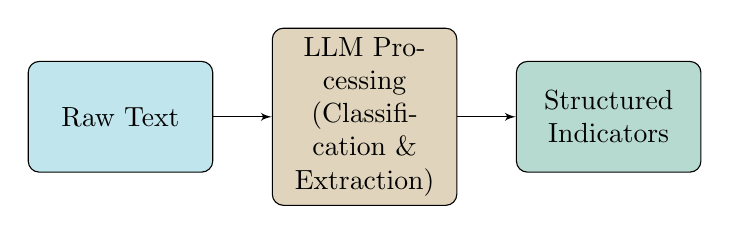
\begin{tikzpicture}[node distance=1.6cm, auto]
                    \tikzstyle{cloud} = [draw, ellipse, fill=red!20, node distance=1.5cm, minimum height=2em]
                    \tikzstyle{block} = [draw, rectangle, fill=blue!20, text width=6em, text centered, rounded corners, minimum height=4em]
                    \tikzstyle{line} = [draw, -latex']
                    
                    \node [block, fill=aauLightBlue!30] (text) {Raw Text};
                    \node [block, right of=text, fill=aauDarkGold!30, xshift=1.5cm] (llm) {LLM Processing (Classification \& Extraction)};
                    \node [block, right of=llm, fill=aauDarkGreen!30, xshift=1.5cm] (indicator) {Structured Indicators};
                    
                    \path [line] (text) -- (llm);
                    \path [line] (llm) -- (indicator);
                \end{tikzpicture}
            \end{block}
        \end{column}
    \end{columns}
\end{frame}

\begin{frame}{Paper 2: How does Modularity Shape Innovation Geography?}
    \begin{block}{Core Idea}
        \alert{We hypothesize that modular technologies thrive under globally-connected support policies, while integral ones require local, cluster-based support.}
    \end{block}
    
    \vfill
    
    \begin{columns}[T]
        \begin{column}{.5\textwidth}
            \textbf{Key Indicators (LLM-Derived):}
            \begin{itemize}
                \item A technology's `modularity score` derived from patent claims and technical specifications.
                \item The geographic distribution of innovation functions (e.g., `knowledge creation`) from news and reports.
            \end{itemize}
        \end{column}
        \begin{column}{.5\textwidth}
            \textbf{Potential Cases / Examples:}
            \begin{itemize}
                \item Green maritime technologies (e.g., modular e-fuels vs. integral ship designs).
                \item Renewable energy systems.
            \end{itemize}
        \end{column}
    \end{columns}

    \vfill
    \textbf{\textcolor{aauDarkGreen}{Analytical Approach:}} Identify a quasi-natural experiment (e.g., a large-scale regulation) to test the hypothesis using causal inference methods.
\end{frame}

\begin{frame}{Paper 3: How Should Policy Evolve with Technology?}
    \begin{block}{Core Idea}
        \alert{We hypothesize that the optimal policy mix shifts after key technical standards are established, moving from R\&D support to market formation.}
    \end{block}
    
    \vfill
    
    \begin{columns}[T]
        \begin{column}{.5\textwidth}
            \textbf{Key Indicators (LLM-Derived):}
            \begin{itemize}
                \item Classification of national `policy instruments` (e.g., `subsidy`, `mandate`) from legal texts.
                \item Tracking `market formation` signals from corporate and news documents.
            \end{itemize}
        \end{column}
        \begin{column}{.5\textwidth}
            \textbf{Potential Cases / Examples:}
            \begin{itemize}
                \item The development of EV charging infrastructure following the OCPP standard.
                \item Smart grid technologies.
            \end{itemize}
        \end{column}
    \end{columns}
    
    \vfill
    \textbf{\textcolor{aauDarkOrange}{Analytical Approach:}} Use the timing of standardization events as an instrumental variable to identify the impact of policy changes.
\end{frame}

\begin{frame}{Paper 4: Do Modular Policy Designs Diffuse Faster?}
    \begin{block}{Core Idea}
        \alert{We hypothesize that policies designed with modular elements—a core objective with adaptable instruments—are adopted more quickly and effectively across countries.}
    \end{block}
    
    \vfill

    \begin{columns}[T]
        \begin{column}{.5\textwidth}
            \textbf{Key Indicators (LLM-Derived):}
            \begin{itemize}
                \item A `policy modularity score` based on the structure and language of the legal text itself.
                \item The `timing of policy adoption` and national adaptation from government documents.
            \end{itemize}
        \end{column}
        \begin{column}{.5\textwidth}
            \textbf{Potential Cases / Examples:}
            \begin{itemize}
                \item Pan-European regulations (e.g., EU Battery Regulation, Digital Services Act).
                \item International climate agreements.
            \end{itemize}
        \end{column}
    \end{columns}
    
    \vfill
    \textbf{\textcolor{aauDarkGold}{Analytical Approach:}} Model the cross-national diffusion process using event-history analysis.
\end{frame}

\begin{frame}{Contribution and Implications}
    \textbf{This research aims to make both a scientific and a practical contribution:}
    
    \vfill
    
    \begin{columns}[T]
        \begin{column}{.48\textwidth}
            \begin{block}{\textcolor{aauDarkBlue}{Scientific Contribution}}
                \begin{itemize}
                    \item Integrates modularity theory with innovation geography and policy studies.
                    \item Develops a novel, scalable method for measuring innovation and policy from text.
                    \item Provides new evidence on the technology-policy interface.
                \end{itemize}
            \end{block}
        \end{column}
        \begin{column}{.48\textwidth}
            \begin{block}{\textcolor{aauDarkGreen}{Policy Implications}}
                \begin{itemize}
                    \item Offers guidance on when to invest locally vs. globally.
                    \item Provides a framework for designing `architecture-aware` innovation policy.
                    \item Informs strategy for critical green technologies.
                \end{itemize}
            \end{block}
        \end{column}
    \end{columns}
\end{frame}

\begin{frame}[allowframebreaks]{References}
    \printbibliography
\end{frame}

\end{document}